\section{Problem statement}
The sections ~\ref{sec:1.1} and ~\ref{sec:1.2} are primarily based on the original TimeTrap paper~\cite{li2024timetrap} and on the lecture notes provided during the Real-Time Kernels and Systems course~\cite{T01},~\cite{T01-dep},~\cite{T06},~\cite{T09},~\cite{T11},~\cite{T14}.
\subsection{Scope of the original work}

\textbf{Introduction to Cyber-Physical Systems (CPS)} \label{sec:1.1} \\
%% T01, Paper in generale
The original work "\textit{An Empirical Study of Performance Interference: Timing Violation Patterns and Impacts}" investigates the use of multi-core platforms in modern Cyber-Physical Systems (CPS) and the safety risks of physical control deviations caused by timing constraint violations. To fully understand the operational context of these systems, we have to take into account the fundamental principles of Cybernetics. A CPS interacts continuously with the physical environment through a strict feedback control loop composed of three continuous phases: \textit{sensing} the external environment, \textit{computing} the required correction, and \textit{actuating} the physical response to reach a system goal.
\\
%% T01, T01-approfondimento, Paper in generale
In the domain of Cyber-Physical Systems and real-time embedded systems, temporal predictability and system dependability are crucial. According to dependability theory, it is essential to distinguish between two of its primary attributes:
\begin{itemize}
    \item \textit{Reliability}, which corresponds to the continuity of correct service delivery:
    \item \textit{Safety}, which corresponds to the non-occurrence of catastrophic consequences.
\end{itemize}  
For a Cyber-Physical System, operational correctness is not determined solely by the result of computation; rather, it also strictly depends on the output's timing, meaning that correctness is evaluated in both the time and value domains. Producing a correct value later than its deadline acts as a fault that degrades the feedback control loop, causing an interruption in the continuity of the expected service (which constitutes a  \textit{reliability issue}). Because a CPS continuously interacts with the physical world, this timing-related reliability failure inevitably translates into a physical deviation (e.g. causing a drone to crash or a robot to deviate from its path), compromising the safety of the physical environment.
\\
%% Paper INTRODUCTION (I) SWaP, Paper (II) Orb Slam
Modern autonomous applications can involve complex software pipelines (e.g. environment perception, localization, and motion planning), which demand huge computational power. To satisfy these requirements while keeping Size, Weight, and Power (SWaP) under strict limits, the embedded industry has heavily migrated to multi-core architectures.
\\
\textbf{Multi-core architectures: Contention for shared resources and performance interference} \\
%% T11, T01, Paper 
Multi-core processors are tightly coupled systems where different cores share physical and logical resources, such as the memory bus, memory controllers, and L2/L3 caches. While this architectural shift successfully scales up average computational throughput, it invalidates the premise that an executing task has exclusive control over the physical hardware. Instead, executing tasks continuously contend for shared architectural resources, destroying the timing determinism of single-core architectures. Because these shared hardware components are primarily designed to optimize average-case performance, they can operate adversarially to the predictability needs of a Real-Time System.
\\
%% Paper INTRODUCTION (I) and Abstract, T11, T05
In the context of Real-Time Systems, this hardware-level access contention generates severe performance interference. 
For example, consider how cache coherence mechanisms are affected in multi-core processors. While individual cores rely on private caches (L1) to minimize memory access latency, tasks running concurrently on different cores often access shared memory locations. This concurrent access can cause local cache contents to diverge, risking the use of obsolete data.
Simultaneous requests to use implicitly shared resources necessitate strict access arbitration. Because of this arbitration, running jobs may hold the CPU without making any actual computational progress; this is called \textit{stalling}. This hidden wait time artificially inflates the \textit{Worst-Case Execution Time (WCET)} of the tasks, demonstrating a critical failure of multi-core environments: the WCET is no longer composable. When applying \textit{Response Time Analysis}, where $R_i = C_i + B_i + I_i$, this hardware interference acts as an unpredictable inflation of the execution time ($C_i$) or as invisible interference ($I_i$), which completely compromises the temporal predictability of the system.
\\
%% Notion (T06)
This hardware-level unpredictability is intensified by how modern real-time software is implemented. To program a real-time system correctly, there must be strict alignment between the programmer's intent (what the system needs to do) and the system rules (the temporal constraints that must be met). However, many programming languages lack native timing semantics, making it difficult to enforce these rules effectively. When developers fail to manage these temporal constraints, hardware-induced delays are allowed to propagate through the software layer.
\\
%% Paper, T09
With a deep analysis of real-world CPS software, the authors of the paper identify that this delay propagation leads to severe \textbf{timing issues} in Cyber-Physical Systems. While similar to conventional concurrency bugs (like data races), these timing issues do not necessarily crash the software; instead, they alter algorithm-level semantics and degrade physical control performance. Through these studies, the authors identify three main vulnerabilities that cause timing issues:
\begin{itemize}[nosep]
    \item \textbf{Type I}: Missing timing constraints. The programmer assumes the timing will be predictable and there is no formal rule in the code to guarantee it;
    \item \textbf{Type II}: Incomplete timing constraints. Timing delays are allowed, but the maximum limits are poorly defined;
    \item \textbf{Type III}: Poorly implemented timing constraints. This is often caused by errors in the system's schedulers or bad coordination between tasks.
\end{itemize}
The combination of multi-core hardware interference and these software vulnerabilities results in \textbf{temporal displacement}. This occurs when critical data becomes misaligned in time, causing the CPS to consume stale or desynchronized data, which can trigger catastrophic failures in the physical world.
\\
%% Paper, T09, T01-approfondimento
\textbf{Mechanism: Temporal Displacement}\\
The paper formulates the potential physical impact of this performance interference through the concept of temporal displacement, which represents the difference between the actual timing of the data update and its expected timing. 
From the perspective of Dependability theory, the progression from hardware interference to physical deviation shows the \textit{Fault → Error → Failure} chain. The targeted performance interference injected into the shared hardware acts as a \textit{fault}. This fault alters the timing behaviour, generating a temporal displacement, which constitutes an anomalous internal system state (\textit{error}). The error manifests in the system's external behaviour as a physical deviation (\textit{failure}).
\begin{figure}[t]
    \centering
    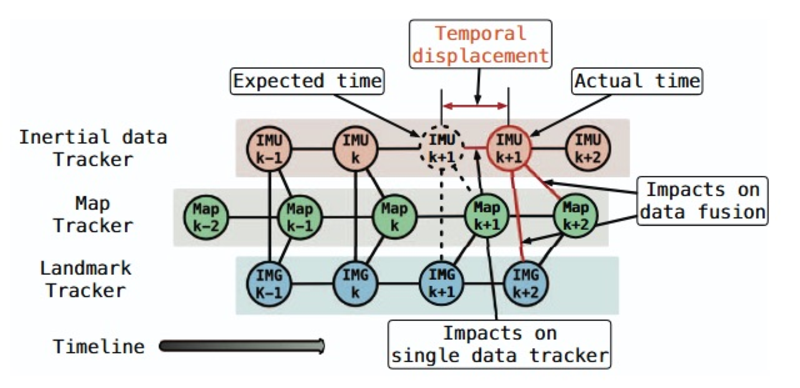
\includegraphics[width=0.80\columnwidth]
        {figures/sensordatatracker.pdf}
    \caption{Temporal displacement. Reproduced from~\cite{li2024timetrap}.}
    \label{fig:sensor}
\end{figure} \\
In modern CPS platforms, tasks do not operate independently; they are organized into processing pipelines, each structured as a transaction that includes a sequence of interdependent tasks. Injecting a delay in a single node, such as a \textit{sensor data tracker} (see Figure~\ref{fig:sensor}), results in a cascading delay that propagates across the entire data flow, causing the error to reach the physical actuators. From the perspective of \textit{End-to-End Analysis}, which evaluates the total timing behaviour across the entire execution pipeline, this dynamic reflects a \textit{producer-consumer dependency} controlled by precedence constraints. A temporal displacement in a producer task introduces a release jitter into the following consumer tasks, such as motion planning or actuation.
This cascading effect desynchronizes the data flow, causing algorithms to evaluate the environment using temporally misaligned data, a condition the authors define as \textit{data misuse}. Ultimately, this dynamic violates the end-to-end deadline, that is the maximum acceptable latency for the entire sensor-to-actuator transaction to complete, and severely degrades the quality of the system's physical response.
\\
It is exactly this vulnerability in the feedback control loop that the authors aim to exploit. While Cyber-Physical Systems typically rely on fail-safe mechanisms to detect severe anomalies and transition the system into a predefined safe operating state, the authors show that targeted timing interference can bypass these mechanisms and cause severe physical deviations in real-world autonomous systems.

\subsection{Purpose of the original work} \label{sec:1.2}
\textbf{Background Literature} \\
% Paper, T01-approfondimento, T14
As explained in the previous section, performance interference in Cyber-Physical Systems is a multi-level issue: it begins with shared hardware contention and finally leads to real-world physical failures.
To fully understand the purpose of the original work, it is necessary to contextualize it within the three distinct lines of research that currently dominate the literature:
\begin{enumerate}[nosep]
    \item \textbf{Hardware-centric research (WCET Analysis)}: It evaluates the maximum extent of worst-case performance interference caused by shared hardware contention. These works successfully quantify the loss of WCET composability and the stalling effects discussed previously. However, they generally evaluate these hardware delays in isolation, without carefully investigating the cascading implications on the overall software behaviour;
    \item \textbf{Software and Scheduling research (End-to-End Analysis)}: It examines the issue from a software perspective. These studies trace the propagation of delays through the execution pipelines, analyzing phenomena like release jitter, increased blocking times, and timing anomalies. So, because this approach focuses purely on the scheduling rules, it often ignores how these OS-level anomalies translate into the machine's real-world physical behaviour;
    \item \textbf{Control Theory and Dependability research}: It focuses on the physical stability of the system. These studies use abstract models to observe how physical control degrades when a task repeatedly misses its deadlines, eventually compromising the system's fail-soft behaviour. Hence, this approach treats deadline misses as theoretical events, failing to link them to their true hardware or OS-level root causes.
\end{enumerate}
These domains are studied as separate problems, introducing the need for a holistic approach.
\\
\textbf{Goal of the paper} \\
The first goal of this work is to bridge this significant research gap. While previous literature has studied hardware timing, software scheduling and control theory in strict isolation, the authors aim to connect them holistically. They want to empirically demonstrate that hardware-level performance interference can induce specific timing violation patterns, such as temporal displacement, which directly propagate through the software pipeline and degrade the physical control outcomes.
\\
From the perspective of Dependability and Error Detection principles, modern Cyber-Physical Systems are typically provided with application-level error detection mechanisms, such as reasonableness checks and data freshness verification. When these built-in mechanisms detect a severe anomaly (e.g. a huge delay in sensor data) the system is programmed to enter a \textit{fail-safe state}. In a fail-safe state, the system maintains its integrity by accepting a temporary halt in its operation or performing a safe, degraded action (e.g. stopping the motors to prevent a crash).
Because of these defense mechanisms, simply saturating the CPU with massive interference is ineffective for an aggressor: this would easily trigger the error detection checks, causing the system to stop safely before any physical damage occurs. 
Hence, the main goal of the paper is to prove that it is possible to design a stealthy timing interference. The authors want to carefully inject delays that are large enough to cause \textit{data misuse} (forcing the system to compute stale data) but small enough to completely bypass the system's error detection mechanisms. In this way, the targeted interference can successfully compromise the control stability and induce severe physical failures.
\\
\textbf{Methodology} \\
To understand how the authors demonstrated their thesis, it is first necessary to examine the inadequacy of conventional attacks. The authors first try a \textbf{simple and direct Denial-of-Service (DoS) attack}, allocating 80\% CPU bandwidth at the highest priority. This type of attack saturates the shared hardware resources with high CPU bandwidth in order to maximize the execution latency of the victim tasks. However, in the context of modern Cyber-Physical Systems, this brute-force approach is ineffective. In particular, inducing this excessive latency leads to the activation of built-in fail-safe mechanisms. In this way, instead of causing control degradation, the system detects the anomaly, halts its operations and then switches to a safe state, preventing any catastrophic physical failure and damage.
The authors also tried a \textbf{"low-bandwidth" DoS attack}, which allocates only a 20\% CPU bandwidth to cause partial resource consumption. While this avoids triggering the immediate fail-safe halt, it only results in a slowdown of the system, like a decreased rate of control output messages or minimal control deviations. The control algorithms are inherently robust enough to gracefully tolerate this minor delay (showing a fail-soft behaviour), allowing the system to maintain its correct physical path without significant deviations.
\\
To overcome the limitations of DoS attacks, the authors introduce TimeTrap. The core logic of this tool is to operate in a stealthy way. The aggressor task is restricted to execute at the lowest priority level in the system and it does not have privileged permissions. Its goal is not to crash the system, but rather to induce targeted jitter and data desynchronization to deceive the system's defenses. The framework operates through the following methodical steps, also shown in Figure~\ref{fig:timetrap}:

\begin{enumerate}[nosep]
    \item \textbf{Exploitable Temporal Displacement Discovery}: TimeTrap utilizes a combination of static analysis and runtime software fault injection. First, it performs static analysis to identify all code regions that access shared data among tasks, classifying them as candidate \textit{delay injection points}. Then, at runtime, it introduces artificial delays at these specific locations. By monitoring the system's physical output, it identifies an effective delay range: a precise temporal displacement that is large enough to corrupt the control algorithms and at the same time small enough to avoid the application's freshness checks and fail-safe mechanisms;
    \item \textbf{Task Execution Phase Breakdown and Interference}: In this phase, TimeTrap performs resource-oriented profiling of the victim task. Since a task utilizes different hardware resources at different times, its execution is broken down into distinct phases based on resource intensity usage. The framework then calculates a \textit{sensitivity curve} to quantify exactly how each phase reacts to the contention of specific architectural channels (e.g. L2/L3 cache, memory bus, disk I/O);
    \item \textbf{Aggressor Workload Generation}: Finally, TimeTrap models the attack generation as a \textit{mathematical optimization problem}. It generates a parameterized workload (the aggressor) shaped to target the victim task during its most vulnerable phase. The objective is to maximize the interference and the resulting delay inflicted on the target, while minimizing the side effects on all other co-running tasks, ensuring the attack remains undetected.
\end{enumerate}
\begin{figure}[t]
    \centering
    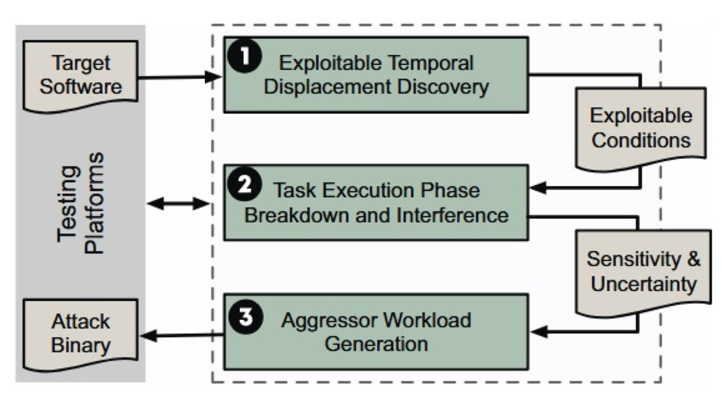
\includegraphics[width=0.80\columnwidth]
        {figures/timetrap.pdf}
    \caption{The workflow of TimeTrap. Reproduced from~\cite{li2024timetrap}.}
    \label{fig:timetrap}
\end{figure}
From a Mixed-Criticality Systems perspective, TimeTrap exposes a limitation of priority-based scheduling:
\begin{itemize}[nosep]
    \item Instead of directly competing for CPU time, the TimeTrap aggressor contends for shared architectural resources, such as caches and the memory bus;
    \item The resulting contention can stall safety-critical tasks, because priority assignment alone does not regulate interference on resources shared across cores;
    \item The attack demonstrates that software-level scheduling alone is insufficient to guarantee temporal isolation. Stronger isolation may be provided through \textit{Time and Space Partitioning (TSP)}, in which a partitioning hypervisor assigns separate execution windows and address spaces to different partitions, complemented by \textit{hardware-enforced partitioning} or regulation of shared resources such as caches and memory bandwidth.
\end{itemize}
Ultimately, this exposes a limitation of integrated multicore platforms: timing predictability cannot rely solely on priority-based CPU scheduling, but also requires explicit control of interference on shared hardware resources.
\\
\textbf{Claims and results} 
\\
The authors evaluated TimeTrap on eight real-world CPS applications using \textit{Hardware-in-The-Loop (HiTL)} simulations and physical tests on the OpenManipulator robotic arm and the Turtlebot3 robot. This allowed for a comprehensive analysis of several stages of the CPS pipeline, such as the perception, localization, planning, and control modules.
\\
The experiments confirmed that direct Denial-of-Service (DoS) attacks generally fail to cause critical physical damage. Both high-bandwidth and low-bandwidth DoS attempts triggered the systems' built-in fail-safe mechanisms or resulted in graceful degradation, such as safely halting the Turtlebot3 or causing only minimal deviations in the robotic arm.
\\
In contrast, TimeTrap successfully bypassed these safety checks by injecting targeted, fine-grained delays. This stealthy temporal displacement induced severe physical consequences: an attack on the robotic arm can cause deviations up to 30.1 cm and a collision; the Turtlebot3 computed incorrect paths based on stale costmaps; an Ardupilot drone showed severe velocity oscillations, leading to a crash.
\\
TimeTrap proved robust across ten different mission tasks, consistently achieving a success rate exceeding 60\% in both static and dynamic scenarios. Its effectiveness was even more pronounced in dynamic environments (reaching an 86\% success rate on the robotic arm), since these scenarios impose stricter timeliness requirements.
\\
Finally, the authors demonstrated that the impact of the attack heavily depends on the targeted shared resource, CPU budget, and task priority. Contention on cache and disk I/O proved significantly more effective than on network I/O, as the former are tightly coupled with the victim's computational phases. Consequently, the resulting temporal displacement scales proportionally with the CPU bandwidth and priority level assigned to the aggressor task.
\\
\textbf{Limitations}\\
The authors also noted several important limitations. First, the success of the attack strongly depends on the physical environment and the current state of the system. Since CPS outcomes are tied to real-world dynamics, the same interference pattern may have different effects depending on if the system is stationary, moving, or operating under changing conditions. In some cases, even a carefully modelled attack may take several seconds to destabilize the system.
\\
The second limitation is mainly constrained to local environments. TimeTrap relies on running the aggressor task on the same computing platform as the victim. This limits the TimeTrap extent compared with a remote attack. However, the authors note that in some systems there might be remotely exposed API that can trigger the interference workload indirectly. In that case, the aggressor would not need direct local code execution because the remote request could invoke a high-priority or resource-intensive path that creates the same kind of timing disruption.

\subsection{Purpose of the assignment}
The purpose of this assignment is not to reproduce the complete TimeTrap framework, but to investigate, on a smaller experimental scale, some of the timing-violation mechanisms and qualitative effects presented in the original paper. A complete reproduction would require automatic injection-point discovery, resource-oriented profiling, sensitivity analysis, and automatic aggressor-workload generation.
\\
Our work instead uses manually selected configurations and controlled perturbations to examine how a timing fault produces an internal temporal anomaly and if this anomaly propagates to control or mission-level behaviour.
The assignment includes two case studies. The \textbf{ArduPilot case study} primarily investigates the effects of different interference mechanisms, including indiscriminate resource saturation, explicit software delay injection, and a low-priority cache-contention workload.
The \textbf{TurtleBot3 case study} introduces explicit delays at different stages of the ROS Navigation pipeline, including localization, TF transmission, local-costmap production, and local-control execution. 
The two case studies do not provide a complete validation of TimeTrap or a general safety assessment. Their objective is to determine if some of the relations between timing perturbation, temporal displacement, data aging, control degradation, and mission-level effects can also be observed in reduced and controlled virtualized environments.
\\
\textbf{Learning objectives}\\ % POI DA DISCUTERNE NELLA PAGINA SELF-ASSESMENT
Through this assignment, we define the following shared learning objectives:
\begin{itemize}[nosep]
    \item \textbf{L0}: Understand the relation between performance interference, timing violations, temporal displacement, data freshness, and control degradation in Cyber-Physical Systems;
    \item \textbf{L1}: Design controlled, repeatable, and measurable real-time experiments using defined configurations, execution procedures, logging mechanisms, and quantitative metrics;
    \item \textbf{L2}: Compare how different perturbation mechanisms and different injection locations affect the timing and control behaviour of a Cyber-Physical System;
    \item \textbf{L3}: Analyze when an internal timing violation remains confined to the targeted software stage and when it propagates to control outputs, physical behaviour, or mission completion;
    \item \textbf{L4}: Critically evaluate if a reduced experimental reproduction supports some of the qualitative claims of the original work, while identifying the limitations introduced by simulation, virtualization, manual injection-point selection, and limited experimental coverage.
\end{itemize}

\subsection{Perimeter of investigation in the assignment}
\\
As introduced before, the complete TimeTrap workflow is beyond the perimeter of this project. The assignment is divided into two experimental case studies. For both case studies, the injection locations, delay values, and aggressor configuration are selected manually to reproduce the small-scale experiment.
\\
\textbf{ArduPilot case study} \\
The ArduPilot experiment is based on the Copter-4.0 version of the ArduPilot codebase. All tests are conducted using its Software-In-The-Loop (SITL) environment. Therefore, the experiment does not involve a physical drone or a flight-control hardware. A predefined mission is used in all configurations to make the different executions comparable and to observe the effects of interference under similar operating conditions.
\\
The ArduPilot case study is guided by the following research questions, which will be addressed in the results and discussion section:
\begin{itemize}[nosep]
    \item \textbf{A-Q0}: Does separating sensor emulation from the control thread change the normal timing and control behaviour of the system compared with the original baseline?     
    \item \textbf{A-Q1}: Does an indiscriminate Denial-of-Service workload mainly increase the wall-clock mission completion time, or does it also cause significant velocity-tracking deviations?
    \item \textbf{A-Q2}: Does targeted delay injection into the control path produce larger control-loop delays, greater navigation-state age, and higher velocity-tracking error than the baseline configurations?
    \item \textbf{A-Q3}: Can a low-priority cache-contention aggressor reproduce, at least qualitatively, the timing and control effects observed with explicit software delay injection?
\end{itemize}
\\ %qui ho dichiarato i 5 esperimenti fatti, segnando per ogni esperimento le research question in cui andrò ad utilizzare i risultati per comparare$
To answer these questions, the study considers both the original SITL architecture and a modified architecture in which sensor emulation is executed in a separate thread. Starting from these configurations, we evaluate the following experimental conditions:
\begin{itemize}[nosep]
    \item \textbf{A-E0}: An execution of the original SITL with logging instrumentation but without interference, which represents the main baseline [A-Q0][A-Q1];
    \item \textbf{A-E1}: An execution of the original SITL under a Denial-of-Service workload [A-Q1];
    \item \textbf{A-E2}: An execution of the modified SITL, with the sensor emulation separated from the control thread but without interference [A-Q0][A-Q2][A-Q3];
    \item \textbf{A-E3}: Two configurations of the modified SITL, with software delays of 30 ms and 50 ms injected into the AUTO waypoint-control path [A-Q2][A-Q3];
    \item \textbf{A-E4}: An execution of the modified SITL under interference generated by a low-priority cache-contention aggressor [A-Q3].
\end{itemize}
\\
The analysis focuses on observable timing and control indicators, including temporal displacement, velocity tracking error, and mission duration. These measurements are used to compare the different configurations and not to provide a complete safety assessment of ArduPilot.
\\
Furthermore, no direct equivalence is claimed between our SITL environment and the hardware-in-the-loop platforms used in the original study, or between the simulation results and the behaviour of the physical drone. The objective is limited to observing if some of the qualitative timing and control effects discussed in the paper can also appear in a smaller and controlled environment.
\\
\textbf{TurtleBot3 case study}\\
The TurtleBot3 case study is based on the ROS Noetic Navigation Stack and uses Gazebo 11 to simulate a TurtleBot3 Burger operating in the \texttt{turtlebot3\_world} environment. The experiments do not involve a physical robot or dedicated embedded navigation hardware. A predefined navigation task is used across the configurations to make the executions comparable and to observe the effects of timing perturbations under similar conditions.
\\
The TurtleBot3 case study is led by the following research questions, which are addressed in the results and comparative-analysis sections:
\begin{itemize}[nosep]
    \item \textbf{T-Q0}: Do the instrumented zero-delay configurations preserve the externally observable command timing and navigation behaviour of the clean TurtleBot3 baseline?
    \item \textbf{T-Q1}: Do controlled software delays produce measurable and increasing temporal displacement or data-age effects at the targeted navigation stage?
    \item \textbf{T-Q2}: To what extent do internal timing violations propagate to the \texttt{/cmd\_vel} stream and mission-level behaviour?
    \item \textbf{T-Q3}: At comparable delay levels, how does the injection location affect timing propagation, navigation availability, and observed safety-related outcomes?
\end{itemize}
To answer these questions, we manually selected injection points at different stages of the ROS Navigation pipeline. Starting from a clean baseline, we evaluated the following experimental configurations:
\begin{itemize}[nosep]
    \item \textbf{T-E0}: An execution of the unmodified ROS Navigation Stack without source-level delay instrumentation, used as the clean navigation baseline [T-Q0];
    \item \textbf{T-E1}: A set of configurations in which a controlled software delay is introduced before the publication of the AMCL pose estimate [T-Q0][T-Q1][T-Q2][T-Q3];
    \item \textbf{T-E2}: A set of configurations in which the AMCL map-to-odometry transform is delayed immediately before its transmission through the TF tree [T-Q0][T-Q1][T-Q2];
    \item \textbf{T-E3}: A set of configurations in which the local-costmap producer task is delayed immediately before updating the map [T-Q0][T-Q1][T-Q2][T-Q3];
    \item \textbf{T-E4}: A set of configurations in which the invocation of the local planner is delayed inside the \texttt{move\_base} control cycle [T-Q0][T-Q1][T-Q2][T-Q3];
    \item \textbf{T-E5}: A set of configurations in which the suspension is introduced at the beginning of the DWA controller execution [T-Q0][T-Q1][T-Q2][T-Q3].
\end{itemize}
Each instrumented experiment includes a zero-delay condition that retains the corresponding source-level timing and logging code without applying an intentional suspension. These conditions are used as matched references for the delayed executions, while T-E0 is used to determine if the instrumentation substantially changes nominal navigation behaviour.
\\
The analysis combines stage-specific internal timing measurements with externally observable navigation indicators.
\\
These measurements are used to compare the timing and behavioural effects of the different injection locations and not to provide a complete safety assessment of TurtleBot3. Moreover, no direct equivalence is claimed between the adopted Gazebo and virtual environments and the physical TurtleBot3 platform evaluated in the original work. The experiments use explicit source-level suspensions rather than TimeTrap-generated resource contention and are conducted in a static simulated environment.
\\
The objective is limited to determining if some of the qualitative temporal displacement and propagation effects discussed in the original paper can also be observed in a smaller and more controlled navigation scenario.
